\subsection{Implementation}
%The process for which metrics, algorithms, and techniques were implemented with the given datasets or input data has been thoroughly documented. Complications that occurred during the coding process are discussed.


As I introduced in the section2.4(Benchmark), I utilized the 4 convolutional layers and 2 fully connected layers.In this section, I explain the architecture of the model in more depth.

The objective of the learning is to minimize the cross entropy in the learning process.
The architecture of the model is the following.

 \begin{figure}[H]

	\begin{center}
	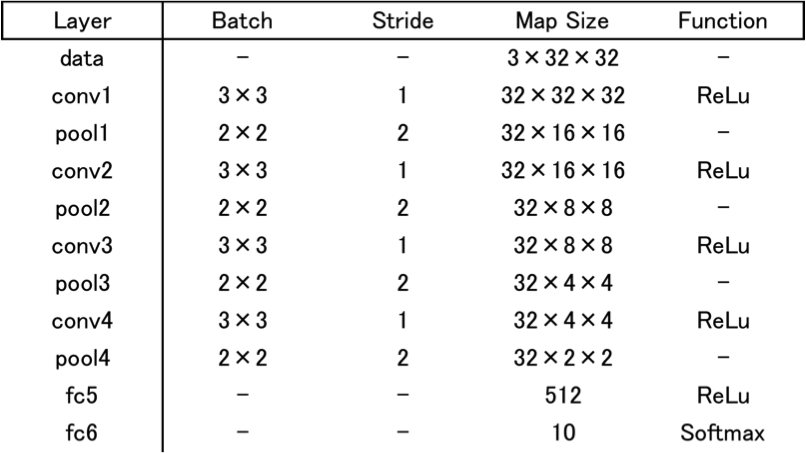
\includegraphics[width=7cm]{picture/layer_architecture.png}
	\caption{Architecture of the model}
	\end{center}
	\label{fig:9}

\end{figure}


As for the optimizer, I utilized 'Adam'.
With this setting, I got the accuracy rate of 70.2\%

To train the CNN model, I used Keras which is one of the neural network libraries like Theano or Tensorflow.

The important parameters training the model is as follows.
Optimization parameters:Learning rate, beta1,beta2, 

The number of stride or map size are shown in Fig.12.
As for the initialization of the random weights in convolutional layers, I used uniform distribution.
I used normalized uniform distribution which is proposed by Glorot\cite{Glorot} for the initialization of the weights in fully connected layers
I used Relu as the activation except for the final layer and I used softmax as the final layer of activation.